\documentclass[12pt,letterpaper]{article}
\usepackage[utf8]{inputenc}
\usepackage{amsmath,amssymb,fullpage,graphicx}
\usepackage{subfigure}
\let\hat\widehat
\let\tilde\widetilde


\author{Nan Tang\\1662478}
	%% your name
\title{STAT 403 Spring 2018\\HW06}
	%% title of this document
\begin{document}
\maketitle
	%% make the title and author

\section*{Q1}
\subsection*{Q1-1}

\subsection*{Q1-2}
\begin{align*}
Var(\bar{X^\star}) &= Var(\frac{1}{n} \sum_{i=1}^{n} X_i ) \text{, since } \bar{X^\star} = \frac{1}{n} \sum_{i=1}^{n} X_i \\
&= \frac{Var(\sum_{i=1}^{n} X_i)}{n^2} \text{, by property of variance} \\
&= \frac{\sum_{i=1}^{n} Var(X_i)}{n^2} \\
&= \frac{Var(X)}{n} \\
\text{Note that  } Var(X) &= \frac{1}{n} \sum_{i=1}^{n} (X_i - \bar{X})^2 \\
Var(\bar{X^\star}) &= \frac{\sum_{i=1}^{n}(X_i - \bar{X})^2}{n^2}
\end{align*}

\begin{align*}
S_n^2 &= \frac{1}{n-1} \sum_{i=1}^{n} (X_i - \bar{X})^2 \\
(n - 1) S_n^2 &= \sum_{i=1}^{n} (X_i - \bar{X})^2 \\
Var(\bar{X^\star}) &= \frac{(n-1) S_n^2}{n^2}
\end{align*}

\noindent As $n \rightarrow \infty$, $\frac{n - 1}{n^2} \rightarrow n$. Therefore, when bootstrap sample size is large enough, variance of bootstrap sample mean is equal to $\frac{S_n^2}{n}$.

\section*{Q2}
\subsection*{Q2-a}
\begin{verbatim}
origin_sd <- sd(faithful$waiting)
bt_size <- 10000
sample_size <- length(faithful$waiting)
bt_result <- rep(NA, bt_size)

for (ii in 1:bt_size) {
  index <- sample(sample_size, sample_size, replace=T)
  bt_dt <- faithful$waiting[index]
  bt_result[ii] <- sd(bt_dt)
}

hist(bt_result, probability=T, col='cornflowerblue', xlab='SD',
     ylab='Density', main='Histogram of Bootstrapped sample SD')
abline(v=origin_sd, lwd=3, lty=1, col='coral1')
\end{verbatim}

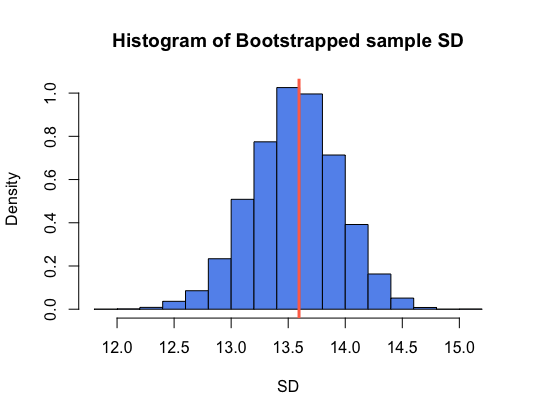
\includegraphics[width=150mm]{hist_bt_sd.png}

\subsection*{Q2-b}
\begin{verbatim}
> sd(bt_result)^2
[1] 0.1472021
> mean((bt_result - origin_sd)^2)
[1] 0.1483897
\end{verbatim}

\noindent Variance of sample SD is 0.1472021, and MSE is 0.1483897.

\subsection*{Q2-c}
\begin{verbatim}
bt_sd <- sd(bt_result)
lower_bd <- origin_sd + qnorm(0.975) * bt_sd
upper_bd <- origin_sd - qnorm(0.975) * bt_sd
> lower_bd
[1] 14.34695
> upper_bd
[1] 12.843

> quantile(bt_result, c(0.025, 0.975))
    2.5%    97.5% 
12.78773 14.29303 
\end{verbatim}

\noindent By theorem, the $95\%$ confidence interval is $[12.843, 14.34695]$. In bootstrap samples, $95\%$ interquantile is $[12.78773, 14.29303]$.

\subsection*{Q2-d}

\begin{align*}
\text{p-value} &= \text{P(getting value more extreme than sample SD} | H0)
\end{align*}

\begin{verbatim}
bt_var <- sd(bt_result)^2
p_value <- 2 * pnorm(origin_sd, 15, bt_var)
> p_value
[1] 1.362628e-21
\end{verbatim}

\subsection*{Q2-e}
\noindent The variance of bootstrapped samples is $\frac{\sigma^2}{n}$, indicating the value will decrease as sample size increases. Larger sample size
minimizes the margin of error, of which small margin of error make the estimation more accurate. 

\section*{Q3}
\subsection*{Q3-a}
\begin{verbatim}
admission_dt <- UCBAdmissions[,,1]

origin_or <- (admission_dt[1,1] * admission_dt[2,2]) / 
  (admission_dt[2,1] * admission_dt[1,2])

## generate dataset based on given information
n_male <- admission_dt[1,1] + admission_dt[2,1]
n_female <- admission_dt[1,2] + admission_dt[2,2]
n <- n_male + n_female

data_pull <- c(rep(1, admission_dt[1,1] + admission_dt[1,2]), 
               rep(0, admission_dt[2,1] + admission_dt[2,2]))

N <- 10000
bt_or <- rep(NA, N)
for (ii in 1:N) {
  sp_index <- sample(n, n, replace=T)
  sp_dt <- data_pull[sp_index]
  sp_male <- sp_dt[1:n_male]
  sp_female <- sp_dt[(n_male+1):n]
  male_admit <- sum(sp_male)
  male_reject <- length(sp_male) - male_admit
  female_admit <- sum(sp_female)
  female_reject <- length(sp_female) - female_admit
  sp_or <- (male_admit * female_reject) / (male_reject * female_admit)
  bt_or[ii] <- sp_or
}

bt_mse <- mean((bt_or - mean(bt_or))^2)

> bt_mse
[1] 0.04906438
\end{verbatim}

\noindent Under bootstrap size of 10000, I get the MSE of OR is 0.04906438.

\subsection*{Q3-b}
\begin{verbatim}
bt_sd <- sd(bt_or)
p_value <- pnorm(origin_or, 1, bt_sd)

> p_value
[1] 0.001652304
\end{verbatim}

\subsection*{Q3-c}


%%% do not touch anything below
\end{document}
